\documentclass[a4paper,14pt]{article}
\usepackage[T1]{fontenc}
\usepackage[utf8]{inputenc}
\usepackage{lmodern}
\usepackage{amsmath}
\usepackage{amsfonts}
\usepackage{amssymb}
\usepackage{amsthm}
\usepackage{graphicx}
\usepackage{color}
\usepackage{xcolor}
\usepackage{url}
\usepackage{textcomp}
\usepackage{parskip}
\usepackage{pdfpages}
\usepackage{hyperref}
\usepackage{float}
\usepackage{enumitem}
\usepackage{subfig}
\usepackage{fancyhdr}
\usepackage{wrapfig}

\renewcommand{\figurename}{Slika}
\graphicspath{ {./img/} }

\title{Operativni sistem Linux}
\author{Aleksa Siriški}
\date{May 2022}

\begin{document}

\pagestyle{empty}
\begin{center}
\textbf{Gimnanzija „Jovan Jovanović Zmaj“}
\\
Novi Sad
\end{center}
\vfill
\begin{center}
	\begin{large}
		\textbf{Maturski rad iz Operativnih Sistema}
		\bigskip 
	\end{large}
	\\
	\begin{huge}
        \textbf{Operativni sistem Linux}
	\end{huge}
\end{center}
\vfill
\begin{normalsize}
Profesor mentor:
\hfill
Učenik:
\\
Saša Tošić
\hfill
Aleksa Siriški IV-6
\end{normalsize}
\vfill
\begin{center}
Novi Sad, maj 2022. god.
\end{center}
\newpage

\pagestyle{plain}
\section{Predgovor}
Za ovu temu sam se opredelio iz više razloga. Prvenstveno zbog ljubavi prema informacionim tehnologijama, koju sam stekao zahvaljujući mojim roditeljima. Drugi razlog je to što smatram da je ovo veoma fascinantna tema, jer obuhvata kompleksnost koje se može postići kada na jednom projektu radi čitav svet. Na kraju, ono što me je privuklo da izaberem baš ovu temu, jeste činjenica da je budućnost IT-a slobodan i besplatan kod.
\\\\
U ovom radu analiziraću osnovne komponente jednog izuzetnog operativnog sistema, istoriju njegove kreacije kao i filozofski pogled na isti.
\newpage

\renewcommand{\contentsname}{Sadržaj}
\tableofcontents
\newpage

\pagestyle{fancy}
\fancyhf{}
\lhead{Operativni sistem Linux}
\rhead{Aleksa Siriški, IV-6}
\cfoot{\thepage}

\section{Istorija\cite{revos}}
MIT u saradnji sa drugim kompanijama su napravili eksperimentalni operativni sistem zvan Multiplexed Information and Computing Service (Multics) 1960. godine. Unics (danas UNIX) su kasnije stvorili i objavili Ken Thompson i Dennis Ritchie  (Slika a) iz AT\&T 1970. godine kao sopstvenu verziju Multics-a. Kasnije je prekucan u C programskom jeziku i time postao veoma fleksibilan i izmenljiv. Razni fakulteti i univerziteti su pravili svoje verzije Unix-a, npr. BSD koji je poput Linuxa i dan danas u upotrebi.
\\\\
Richard Matthew Stallman (Slika b), osnivač GNU projekta\cite{gnu}, je uz svoj tim započeo izradu kompletnog operativnog sistema čija je glavna namena  bila da bude otvorena i slobodna alternativa za Unix. Jedina stvar koja je falila jeste kernel, sto je jezgro operativnog sistema koje služi da poveže sve druge komponente u zajednicu.
\\\\
Linus Torvalds (Slika c) koji je bio isprovociran nedostatkom kernela za potpuno slobodan i otvoren operativni sistem odlučuje da napiše svoj sopstveni. Već je bio upućen u Minix i GNU softver te je tokom studija u Finskoj započeo projekat nazvan "Linux" (Slika d). U početku je jedini radio na njemu, ali do danas se priključilo preko 15000 programera u kreiranju kernela koji se sastoji iz vise od 17 miliona linija koda\cite{linuxfoundation}.
\\\\
\begin{figure}[h]
	\centering
    \subfloat[Ken Thompson i Dennis Ritchie, tvorci Unix-a]{{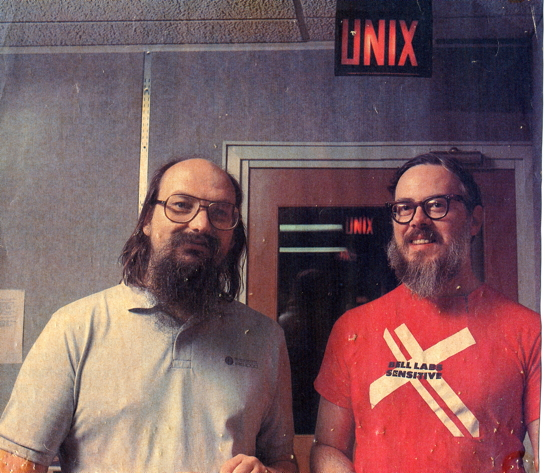
\includegraphics[height=3cm,width=4cm]{ken-thompson-dennis-ritchie} }}
    \hspace{1cm}
    \subfloat[Richard Matthew Stallman, tvorac GNU-a]{{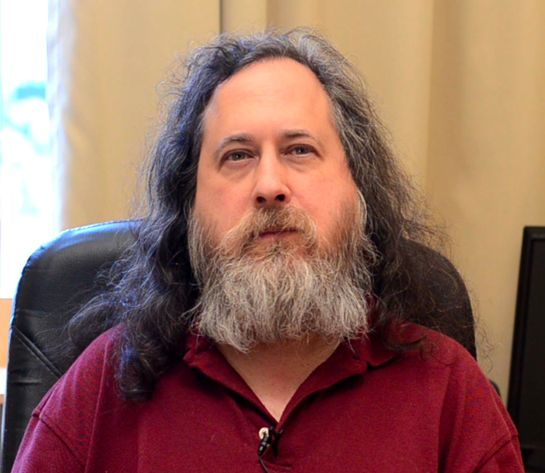
\includegraphics[height=3cm,width=4cm]{richard-stallman} }}
    \hspace{1cm}
    \subfloat[Linus Torvalds, tvorac Linux-a]{{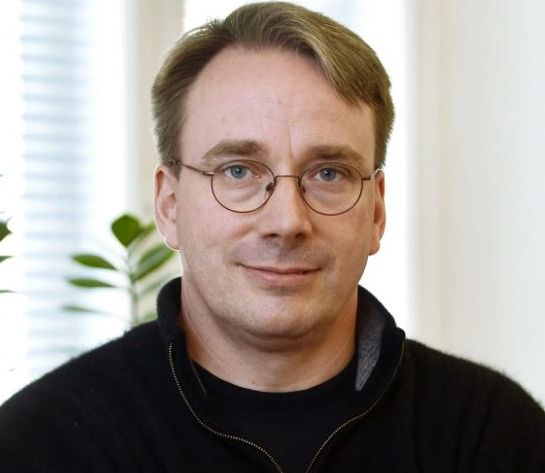
\includegraphics[height=3cm,width=4cm]{linus-torvalds} }}
    \hspace{1cm}
    \subfloat[Linux logo]{{
\includegraphics[height=3cm,width=4cm]{linux} }}
\end{figure}
\newpage

\section{Distribucije}
GNU/Linux operativni sistem se može samostalno napraviti kompajliranjem svih potrebnih programa (npr. Linux From Scratch), ali se najčešće koriste već gotove distribucije. Sve distribucije dele jednu stvar, Linux kernel, ali po svemu ostalom se mogu potpuno razlikovati, doduše većina distribucija ima neke zajedničke osnovne komponente.
\\\\
Postoje distribucije pravljene za servere:
\begin{itemize}
\item Debian (Slika a)
\item Ubuntu server
\item CentOS
\item Turnkey
\end{itemize}
Kao i distribucije pravljene za desktop korisnike:
\begin{itemize}
\item Ubuntu (Slika b)
\item Linux Mint
\item PopOS
\item Fedora Workstation (Slika c)
\end{itemize}
Takođe postoje minimalne distribucije pravljene za kontejnere:
\begin{itemize}
\item Alpine Linux (Slika d)
\item Fedora CoreOS
\item openSUSE MicroOS
\end{itemize}
\begin{figure}[h]
	\centering
    \subfloat[Debian]{{
\includegraphics[height=3cm,width=3cm]{debian} }}
    \subfloat[Ubuntu]{{
\includegraphics[height=3cm,width=3cm]{ubuntu} }}
    \subfloat[Fedora]{{
\includegraphics[height=3cm,width=3cm]{fedora} }}
    \subfloat[Alpine]{{
\includegraphics[height=3cm,width=3cm]{alpine} }}
\end{figure}
\newpage

\section{Komponente}
\subsection{Kernel}
Kernel\cite{kernel} je najvažniji deo svakog operativnog sistema. Služi da pokrene svaku komponentu koja je potrebna za korišćenje OS-a kao i da dozvoli komunikaciju softvera sa hardverom, ili jednog softvera sa drugim. Kernel je neophodan da bi operativni sistem funkcionisao i kao takav je ključno da je minimalan i efikasan.

\subsubsection{Kategorije kernela\cite{kernelcats}}
\begin{itemize}
\item Monolitski - ovde se nalaze svi servisi operativnog sistema se nalaze i izvršavaju se u prostoru samog kernela. Ima zavisnosti između sistemskih komponenti i ogromne količine linija koda što ga čini veoma kompleksnim.
\begin{itemize}
\item Unix
\item Linux
\item Open VMS
\item XTS-400
\end{itemize}
\item Mikrokernel - minimalistički, ima virtualnu memoriju i raspoređivanje niti (eng. \textit{thread scheduling}). Samim tim što je manji je i stabilniji, ali zato ima mnogo više sistemskih poziva jer stavlja sve druge procese u korisnički prostor.
\begin{itemize}
\item GNU Hurd
\item Mach (MacOS)
\item L4
\item AmigaOS
\item Minix
\item K42
\end{itemize}
\item Hibridni - mešavina monolitskog i mikro kernela. Ima brzinu i dizajn monolitskog ali modularnost i stabilnost mikrokernela.
\begin{itemize}
\item Windows NT
\item Netware
\item BeOS
\end{itemize}
\item Egzokernel - prati end-to-end princip, ima najmanju apstrakciju hardvera i direktno dodeljuje fizičke resurse aplikacijama.
\item Nanokernel - samo apstrakcija hardvera, bez sistemskih servisa. Veoma sličan mikrokernelu.
\end{itemize}
\newpage

\subsubsection{Osnovni delovi Linux kernela\cite{devibm}}
\begin{itemize}
\item Menadžer procesa - kao što mu ime implicira, služi da rukuje procesima tj. programima. Svaki proces je zapravo svoj virtualni procesor, nazvan nit. Programi mogu alocirati više niti, takozvanih "radnika". Termin "proces" i "nit" su istog značenja, mada je "proces" više popularan u Desktop aplikacijama.
\item Menadžer memorije - memorija u Linuxu je programima predstavljena kao gomila stranica koje su potom multiplicirane i dodeljivane po zahtevu tog programa. Standard su stranice od 4KB. Takođe, stranice je moguće prebaciti sa sistemske RAM memorije na hard disk, takav postupak se naziva \textit{swapping}.
\item Drajveri - kod koji čini najveći deo linux kernela, omogućava korišćenje određenog hardvera.
\item Virtualni sistem datoteka (VFS) - apstraktuje osnovne komande za manipulaciju podataka čime omogućava korišćenje raznovrsnih sistema datoteka.
\end{itemize}
\newpage

\subsection{Bootloader}
Bootloader je program koji se pokreće pre samog operativnog sistema. Omogućava izbor između više operativnih sistema (dual boot), kao i izbor između različitih kernela na istom operativnom sistemu. Najpre se pokreće kernel, zatim mikrokod procesora (npr. intel-ucode, amd-ucode) i na kraju inicijalni memorijski disk (\textbf{init}ial \textbf{ram} \textbf{f}ile\textbf{s}ystem). Takođe, u bootloader-u se definišu dodatne i zamenjive opcije za kernel.
\subsubsection{Bootloader-i sa podrškom za Linux}
\begin{itemize}
\item \textbf{GR}and \textbf{U}nified \textbf{B}ootloader - najpopularniji zbog velike podrške za svakakve sisteme, jedini podržava enkriptovanu boot particiju. Nastao kao deo programa za GNU operativni sistem.
\item rEFInd - nastoji da ima što više opcija kao GRUB ali sa manjim i jednostavnijim konfiguracijama.
\item systemd-boot - deo systemd, veoma jednostavan i minimalan.
\item EFISTUB - metoda umetanja Linux kernela kao samostalnog bootloadera u novije UEFI BIOS sisteme.
\end{itemize}

\subsection{Daemons}
Demoni\cite{daemon}, naziv nastao od Maxwell-ovog demona koji u pozadini sortira molekule, služe da rade baš to: u pozadini postoje bez korisničkog interfejsa i čekaju na neki događaj i da nude usluge.

\subsection{initramfs}
Init je prvi program koji se pokreće nakon kernela, automatski postaje roditelj svakog narednog programa i poslednji se zaustavlja pri gašenju računara. Kao takav, služi da omogući pristup fajl sistemima, da reguliše demone i snabdeva informacije o njima.
\subsubsection{Init sistemi sa podrškom za Linux}
\begin{itemize}
\item systemd - najpopularniji ali i najobimniji, ne prati KISS (\textit{keep it simple, stupid}) jer integriše mnogobrojne dodatne funkcionalnosti kojim init sistem ne bi trebao da se bavi.
\item OpenRC - prvi izbor za one koje ne vole systemd, minimalan i brz.
\item GNU Shepherd - Nastao kao deo programa za GNU operativni sistem.
\item BusyBox - nastao za korišćenje na ugrađenim slabim uređajima (eng. \textit{embedded devices}).
\item runit - UNIX init sistem, zamena za SysVinit.
\item SysVinit - tradicionalni init sistem.
\end{itemize}
\newpage

\subsection{Shell}
Ljuska (eng. \textit{shell}) služi da korisniku pruži isključivo tekstualni interfejs, naziv "ljuska" upućuje da je to spoljni deo operativnog sistema. Korisnik unosi komande i dobija odgovore. Osim pokretanja programa, shell može da koristi izlaz jedne komande kao ulaz druge, što se naziva \textit{piping} (prvo uveden u UNIX-u). Takođe može da se koristi i kao programski jezik pri pisanju shell skripti.
\subsubsection{Shell-ovi sa podrškom za Linux}
\begin{itemize}
\item bash - najpopularniji i standard za većinu distribucija, brz i jednostavan. Nastao kao zamena za sh.
\item zsh - obimniji i sporiji, najpre se koristi radi automatskog završavanja pri unosu komandi i sugestije istih.
\item fish - sličan zsh-u, jednostavniji za konfiguraciju ali nije POSIX (neke osnovne komande se razlikuju od većine drugih shell-ova)
\item sh - UNIX shell
\item dash - minimalan i efikasan, nastao isključivo da pokreće POSIX skripte. Četiri puta brži od bash-a, ali nije pravljen za direktno korišćenje u terminalu.
\end{itemize}

\subsection{Display server}
Displej server služi da omogući prikaz GUI-a korisnicima koristeći WIMP (prozori, ikonice, meniji, pokazivač kursora) paradigmu za korisnički interfejs. Svaka aplikacija dobija svoj prozor izmenljive veličine, najčešce pravougaonog oblika.
\subsubsection{Display serveri sa podrškom za Linux}
\begin{itemize}
\item X, X11 ili XOrg - prvi i najkorišćeniji displej server za UNIX-oidne sisteme. Nastao pre više od 30 godina i još uvek u upotrebi zbog spore adopcije drugih protokola. Zahteva dodatan kompozitor za bilo kakve efekte (npr. providnost prozora) i VSync.
\item Wayland - nastao u cilju da bude moderna alternativa za X pre više od 10 godina, ali je tek u proteklih par godina počeo eksponencionalno da se razvija i danas je standard na samo par distribucija (Fedora, Ubuntu, openSUSE, Debian). Drastično povećava bezbednost time što dodaje kontrolu dozvola aplikacijama, za razliku od X gde svaka aplikacija može da vidi jedna drugu. Wayland nema dodatne kompozitore, već je svaka primena Wayland protokola sama svoj kompozitor.
\end{itemize}
\newpage

\section{Komande}
Jedna od velikih prednosti Linux operativnog sistema jeste terminal, kojim je omogućena upotreba kompletnog korisničkog interfejsa. Tek je naknadno ubačena podrška za grafički korisnički interfejs.
\subsection{Osnovne komande u Linux terminalu}
\begin{itemize}
\item pwd - ispisuje trenutni direktorijum u kom se nalazi i u kom će se izvršavati sve komande. Inicijalni terminal je kućni folder korisnika koji ga pokreće.
\item ls - ispisuje sve foldere i fajlove u zadatom direktorijumu. U slučaju skrivenih foldera i fajlova koristi se \textbf{ls -a}.
\item cd - menja trenutnu lokaciju tj. folder.
\item mv - pomera fajl.
\item cp - kopira fajl.
\item mkdir i rmdir - pravljene i brisanje foldera.
\item touch i rm - pravljenje i brisanje fajlova.
\item cat - ispis svega što se nalazi unutar fajla.
\item man - ispisuje uputsva jedne komande.
\item sudo - \textbf{S}uper \textbf{U}ser \textbf{DO} - pokreće komandu kao root korisnik.
\end{itemize}
\newpage

\section{Hijerarhija sistema datoteka}
Na Linux operativnom sistemu sve je predstavljeno kao fajl - jezgra procesora, sistemski diskovi, čak i tastatura i miš. Hijerarhija sistema datoteka (FSH) definiše strukturu foldera. Sve se nalazi unutar glavnog root foldera i pristupa mu se kosom crtom.
\subsection{Glavni direktorijumi Linux sistema datoteka}
\begin{itemize}
\item bin - neophodni programi za pokretanje sistema - mount, ls, cp.
\item boot - neophodni fajlovi za pokretanje sistema - kernel, initramfs, mikrokod procesora.
\item dev - uređaji predstavljeni kao fajlovi - hard diskovi, procesor, grafička kartica.
\item etc - konfiguracioni fajlovi za sistemske programe.
\item home - folderi i fajlovi svih korisnika na sistemu sa izutetkom glavnog korisnika na /root.
\item lib - biblioteke potrebne za pokretanje programa iz /bin.
\item media - mesto za priključne medije, npr. usb flash, CD.
\item mnt - slično /media, namenjeno za pristup privremenim uređajima.
\item proc - informacije o sistemskim procesima i kernelu u obliku fajlova
\item tmp - privremeni fajlovi koji se brišu pri gašenju računara
\item usr - primarni direktorijum za izvršavajuće programe na sistemu
\item var - promenljivi fajlovi koji zapisuju promene i podatke tokom izvršavanja programa
\end{itemize}
\newpage

\section{Dozvole i vlasništvo}
Linux operativni sistem za svaki objekat, tj. fajl ili folder, ima određene dozvole. Moguće ih je videti komandom \textbf{ls -l}. Postoje tri vrste dozvola: čitanje, pisanje i pokretanje. Takođe postoje tri vrste vlasništva: vlasnik, grupa i svi ostali. Na ta tri vlasnišva se određuje koje dozvole imaju, koristeći sledeće brojeve:
\begin{itemize}
\item 0 - nema nikakvih dozvola
\item 1 - dozvola za pokretanje
\item 2 - dozvola za pisanje
\item 3 - dozvola za pokretanje i pisanje
\item 4 - dozvola za čitanje
\item 5 - dozvola za čitanje i pokretanje
\item 6 - dozvola za čitanje i pisanje
\item 7 - ima sve dozvole
\end{itemize}
Dozvole nekog fajla ili foldera se menjaju komandom \textbf{chmod} a vlasništvo komandom \textbf{chown vlasnik:grupa}.

\section{Okruženja radne površine}
Okruženja radne površine su skupovi programa koji omogućavaju korišćenje grafičkog interfejsa. Čine ih razne komponente kao što su menadžer prijava, zaključavajući ekran, tekstualni editor i najvažnije menadžer prozora. Moguće imati samo menadžer prozora i zasebno skidati sve druge potrebne programe za korišćenje grafičkog interfejsa ali korišćenje kompletnog okruženja drastično pojednostavljuje taj proces.
\subsection{Desktop okruženja sa podrškom za Linux}
\begin{itemize}
\item GNOME\cite{gnome} - GNU okruženje sa podrškom za Wayland, najpopularniji izbor za distribucije. Nastao kao deo programa za GNU operativni sistem.
\item KDE Plasma\cite{kdeplasma}  - drugo najpopularnije okruženje, takođe sa podrškom za Wayland. Nastao kao više izmenljivo okruženje koje je meri sa GNOME koji ima specifični filozofski pogled na način upotrebe računara.
\item Xfce\cite{xfce} - modularno i nezahtevno okruženje.
\item LXQt\cite{lxqt} - okruženje koje koristi najmanje resursa.
\item MATE\cite{mate} - započet kao klon GNOME 2 kada je GNOME prešao na verziju 3, ali sada i sam koristi tu verziju.
\item Cinnamon\cite{cinnamon} - standardno okruženje za Linux Mint, nastoji da olakša prelazak sa Windows okruženja.
\end{itemize}
\newpage

\section{Kontejnerizacija}
Kontejnerizacija je jedna od jačih strana Linux operativnog sistema. Mogućnost izolacije programa od ostatka sistema sa minimalnim gubitkom performansi je razlog zašto je Linux izbor za najveći procenat servera. Za razliku od virtualnih mašina, kontejneri dele kernel sa domaćim operativnim sistemom i time štede na veličini.
\subsection{Vrste kontejnerskih okruženja}
\begin{itemize}
\item Linux kontejneri\cite{lxc} - najprostiji vid korišćenja kontejnera na Linuxu, pomoću cgroups iz kernela omogućeno je kreiranje više kontejnera na jednom domaćinu.
\item Docker\cite{docker} - komercijalizovan i besplatan softver za manipulaciju kontejnera. Najpopularniji na tržištu.
\item Podman\cite{podman} - RedHat-ova alternativa za docker, nastoji da bude sintaksno identična ali ne zahveta root dozvole za razliku od Docker-a.
\item Flatpak\cite{flatpak} - RedHat-ova jednostavna distribucija desktop aplikacija korišćenjem kontejnera. Developeri mogu predvidljivo da prave kontejner pored sopstvene aplikacije i tako osiguravaju da će se ona identično ponašati ne zavisno od domaćinskog operativnog sistema. Usput pruža ogromna poboljšanja za bezbednost u vidu dozvola (slično Android-u).
\item Snap\cite{snap} - Canonical-ova distribucija aplikacija, slična flatpak-u ali trenutno mnogo sporija. Serverska strana im je centralizovana i zatvorenog koda.
\item AppImage\cite{appimage} - nastoji da olakša distribuciju aplikacije kao flatpak i snap, ali nema jedno mesto na kom se traže aplikacije, već developeri sami prave i distribuiraju nalik običnim pokretljivim datotekama (.exe, .deb, .rpm). Svaka aplikacija dolazi uz svoj skup biblioteka i programa potpuno izolovanih, što bespotrebno troši memoriju, ali je lakše za održavanje.
\end{itemize}
\newpage

\section{Zaključak}
Linux operativni sistem je prvi izbor za najveći broj servera, ali je takođe i korišćen u raznim naučnim i obrazovnim institucijama. Uprkos tome što se bazira na besplatnom modelu postojanjem kompanija kao što su RedHat i mnoštvom sponzora (Microsoft, Google, Facebook/Meta) Linux nastavlja dalje da se eksponencijalno razvija. Ljudi koji se bave programiranjem Linux-a imaju platu kao kad bi radili na identičnom proizvodu zatvorenog koda, što dokazuje da je etika slobodnog koda uspešna i da ne postoji razlog za zatvorenim kodom osim prikupljanja personalnih podataka bez javnog priznanja o tom postupku. Važno je napomenuti da ako je nešto "otvoren" kod ne znači i da je "slobodan" kod. Otvoren kod dozvoljava svakome da vidi tačno šta se izvršava u programu ali mu ne daje na pravo da radi sa tim kodom šta god poželi, dok slobodan kod omogućuje svakome da ponovo koristi taj kod za nešto potpuno drugo ako će takođe dozvoliti ponovnu upotrebu tog novonastalog koda što drastično smanjuje potrebnu za pisanjem istog koda iznova. Da bi se sprečila krađa koda i zloupotreba Stallman je osmislio licence za otvoren i slobodan kod (npr. GNU General Public License\cite{gpl}).
\\\\
Najčešće neuočljivo ali Linux je prisutan u velikom broju svakodnevnih uređaja. Najpopularniji je Android operativni sistem za pametne telefone koji koristi Linux kernel kao i pametni televizori (npr. Samsung-ova odluka da nove modele televizora preinstalira sa Tyzen-om, Linux distribucijom, umesto AndroidTV-a). U današnje vreme i prosečni korisnik koji nije i ne želi da bude upućen u kompleksne tokove rada računara može vrlo jednostavno da koristi Linux upotrebom gotovih distribucija i usput pokrene većinu Windows programa zahvaljujući sloju kompatibilnosti WINE i VALVE-ovim PROTON. Brzinom razvoja i rasprostanjenošću podrške hardvera i softvera vrlo je verovatno da će u bližoj budućnosti Linux zameniti i trenutno glavne Desktop operativne sisteme.
\newpage

\renewcommand\refname{Literatura}
\bibliographystyle{unsrt}
\addcontentsline{toc}{section}{Literatura}
\bibliography{literatura}
\newpage

\section{BIOGRAFIJA MATURANTA}
\begin{wrapfigure}{r}{0.35\textwidth}
\centering
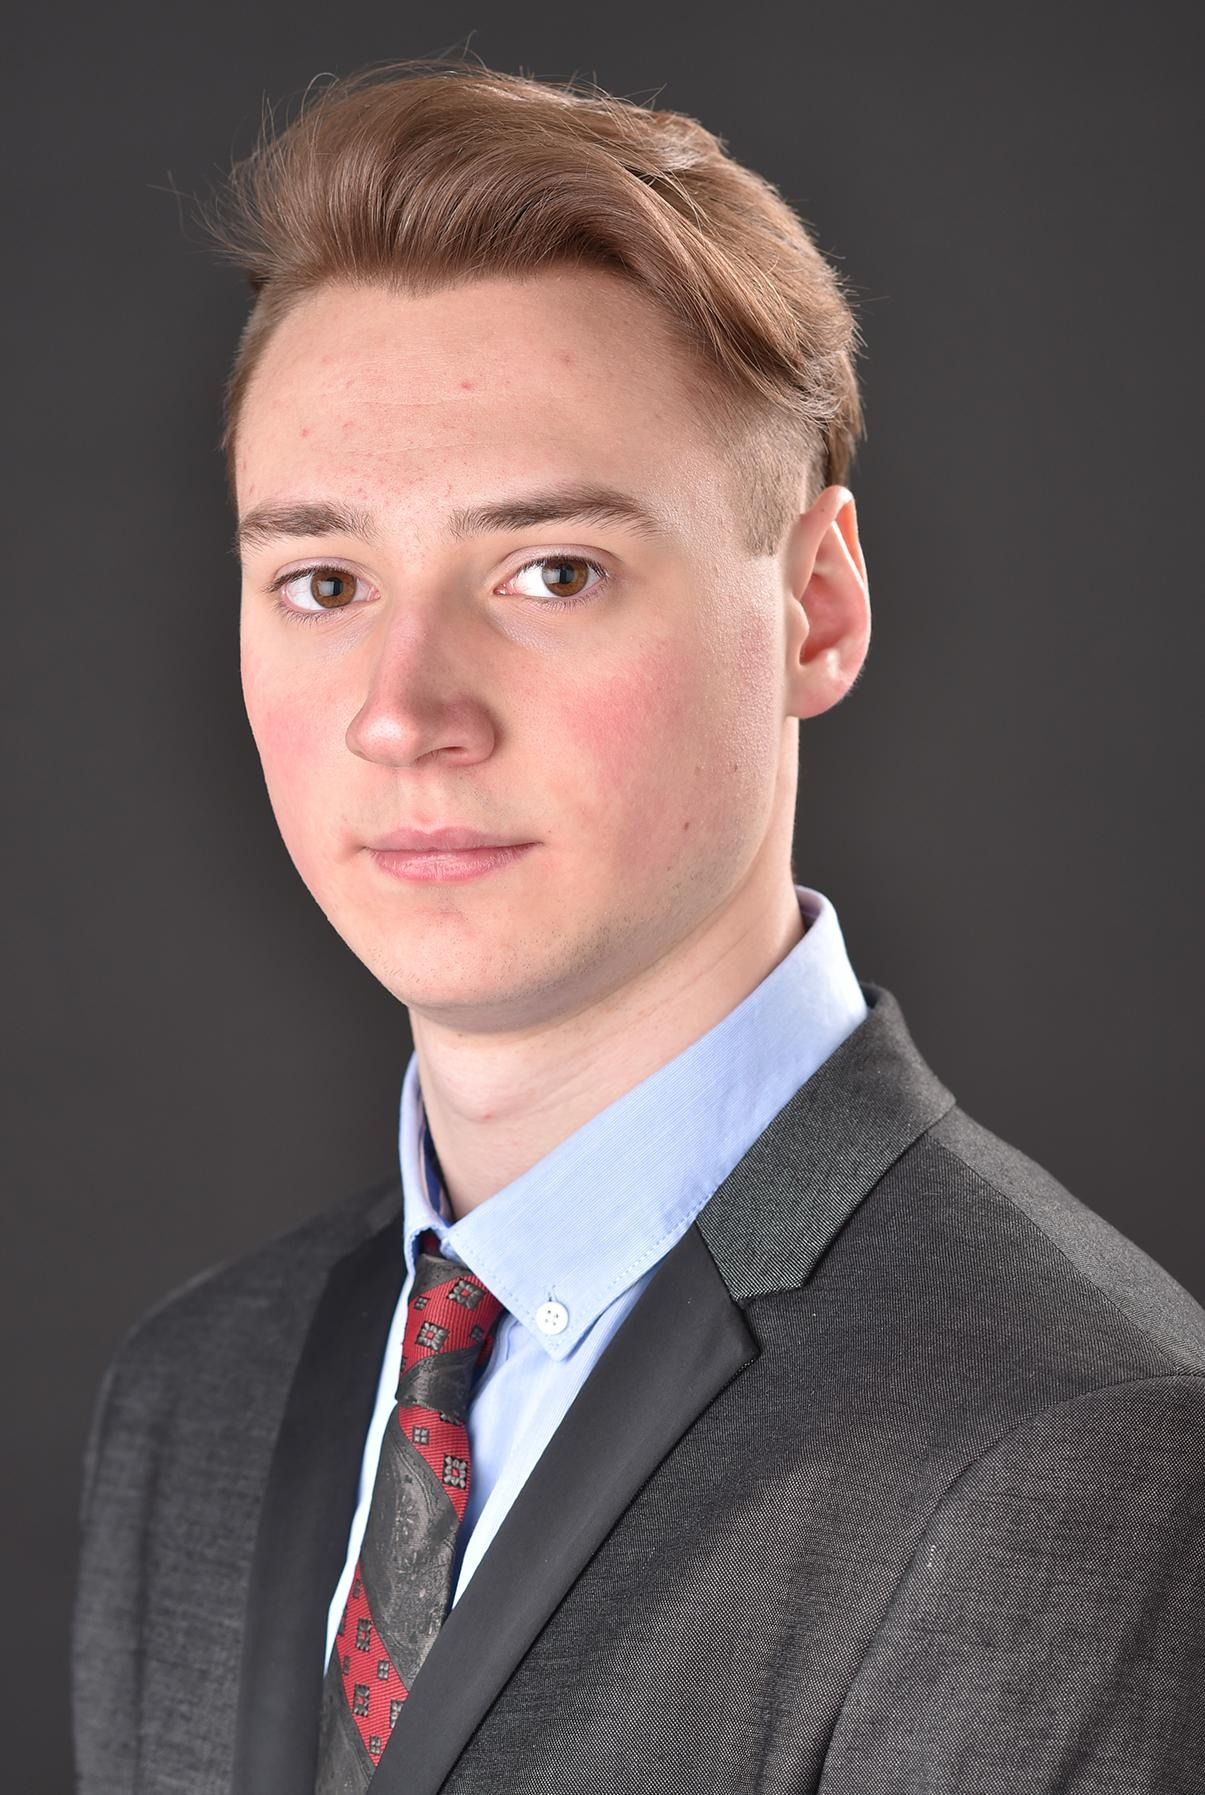
\includegraphics[width=.90\linewidth]{Maturska}
\end{wrapfigure}
Aleksa Siriški rođen je 10. jula 2003. godine u Novom Sadu. Pohađao je Osnovnu školu „Svetozar Marković Toza“ do šestog razreda. Tamo stiče interesovanje za matematiku, informatiku, fiziku i jezike. Septembra 2016. upisuje Osnovnu školu pri Gimnaziji „Jovan Jovanović Zmaj“, kako bi intenzivnije radio u oblastima matematike, fizike i informatike. Istovremeno pohađa programerski kurs „Centar za mlade talente“. Školovanje nastavlja u istoj gimnaziji i opredeljuje se za smer „Učenici sa posebnim sposobnostima za računarstvo i informatiku“. Naredne četiri godine, uporedo sa školom, pohađa i kurseve engleskog i nemačkog jezika. Planira da više obrazovanje stekne na Prirodno matematičkom fakultetu, smer Informacione tehnologije.
\newpage

\end{document}